%%%design overview over libpninx

The aim of \pninx\ is to provide an easy to use but yet powerful interface
to write Nexus files from C++. Although the Nexus group already provides 
an binding of their Nexus API (NAPI) for C++, this is not much more than a 
thin wrapper around the Nexus C API. Thus the native C++ API does not espose
many of the features a C++ programmer would expect from an API. 
\pninx\ is an approach to overcome the limitations of the native C++ API 
and provide you with all the object oriented features that C++ exposes.

This chapter presents the general design of the API. Every user of the API is
highly encouraged to read this chapter as it contains the basic information 
required to use the API. In particular 
section~\ref{section:nxfield_design} should be read by all users of \pninx. 

\section{Nexus and HDF5}

There is some confusion about how Nexus and HDF5 are related to each other. 
The reason for this confusion is mostly due to the fact that Nexus is considered
by many people to be a physical file format of its own. Indeed, Nexus is only a
set of rules and conventions how data should be organized (we will see later
what this means). However, in the end data is writing using one of several
physical file formats supported by Nexus. These formats are XML, HDF4, and last
but not least HDF5. As Nexus describes the structure of data (not the way how it
will be stored on disk) the file format used to store data according to the
Nexus standard must provide some kind of structuring mechanisms as it is the
case for the formats mentioned above. 
While the native Nexus APIs support all these physical file formats \pninx\
only supports HDf5. However, as the other tow (HDF4 and XML) are available
mostly due to historical reasons, this is not a serious limitation. 

HDF5 is a binary file format which is primarily developed  to store large
amounts of numerical data. 
An HDF5 file can be considered pretty much like file system. The data is stored 
in objects called {\em datasets}. In simplest case a dataset is a
multi-dimensional array holding data of a particular type. The datasets can be 
organized in {\em groups}. Thus, to come back to the image of a file system 
the datasets represent files where the groups can be considered as directories.
For those who are more familiar with scientific software development a dataset
can also be imagined as a {\tt numpy} array in Python or as a numerical array 
in Fortran. Such arrays have a data-type and a shape. The later one holds the 
number of elements along each dimension of the array.
As the datasets are organized by groups each of them can be addressed by a Unix
like path (we are back again in the file-system picture). In the 

Attributes can be attached to groups and datasets in an HDF5 file. One  can
imagine attributes as kind of tags that can be stuck on an object. 
Attributes by them self can be strings, arrays or whatever other data you might 
can think of. 


\section{Classes and implementation}\label{section:classes_implementation}

%%%----------------------------------------------------------------------------
\begin{figure}[tb]
\centering
\begin{minipage}[t]{0.4\linewidth}
\centering
\resizebox{\linewidth}{!}{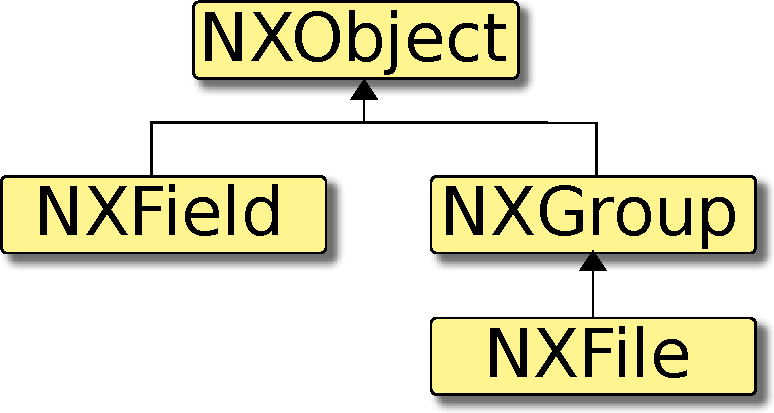
\includegraphics{pics/class_inheritance.pdf}}
\caption{{\small\label{fig:class_inheritance}
There are only four major objects: \nxobject, \nxfield, \nxgroup, and 
\nxfile. Which are all derived from \nxobject. 
}}
\end{minipage}
\hfill
\begin{minipage}[t]{0.59\linewidth}
\centering
\resizebox{\linewidth}{!}{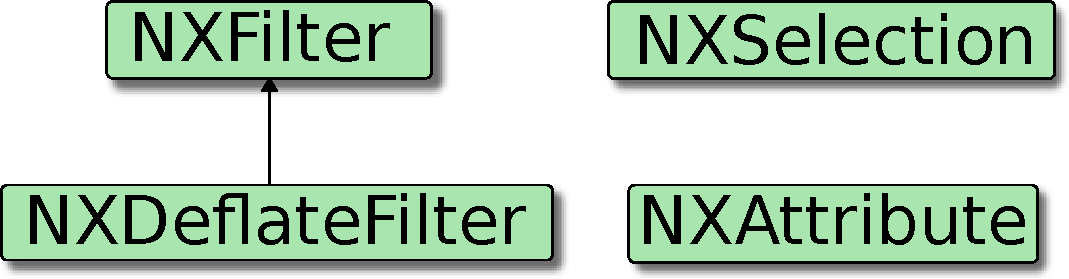
\includegraphics{pics/helper_classes.pdf}}
\caption{{\small\label{fig:helper_classes} 
Utility classes: \nxfilter\ and its only implementation \nxdeflate\ allow data
compression. \nxselection\ implements partial IO and \nxattribute\ manages the
access to attribute data attached to instances of \nxobject\ and its
descendants.
}}
\end{minipage}
\end{figure}
%%%----------------------------------------------------------------------------
One of the design goals behind \pninx\ was to keep things as simple as possible.
Thus the number of classes a user must remember and actually the total number of
classes available was kept as small as possible. 
There are three major classes which are responsible for reading, writing, and
structuring data:
\begin{description}
\item[\nxgroup] the standard container to hold all kinds of objects
\item[\nxfield] the data holding objects
\item[\nxfile] object representing a data file.
\end{description}
As shown in Fig..~\ref{fig:class_inheritance} all these classes are derived from
\nxobject which provides the functionality shared by all classes (attribute
management, inquiry, etc.).
The three classes mention in the enumeration above can be subdivided into two
types of classes: structuring components to which \nxgroup\ and \nxfield\
belong, and data holding objects represented by the single \nxfield\ class.

Along with these fundamental classes come several utility classes shown in 
Fig.~\ref{fig:helper_classes}. \nxfilter\ is the base class for all filter
objects that allow compression of data stored in an instance of \nxfield. 
Actually only \nxdeflate\ filter is available which applies a deflate filter (as
known from {\tt zlib}) on the data. \nxselection\ allows access to parts of the
data stored in an \nxfield\ object. It thus mimics the behavior of selections in
the HDF5 world. \nxattribute\ finally manages the access to attributes attached
to instances of \nxobject and its descendants.

In order to make the API independent of the concrete implementation a Bridge
pattern was used for the implementation of all classes (see~\cite{book:gof}).
However, the intention was not to provide more physical file formats like XML
but rather to easily handle improvements and new APIs for HDF5 without 
influencing user code. This should help making maintenance of \pninx\ easier.

\section{Supported datatypes}
%%%----------------------------------------------------------------------------
\begin{table}[tb]
\centering
\begin{tabular}{l|c|l||l|c|l}
 name & size (Bit) & description & name & size (Bit) & description \\
 \hline
 {\tt UInt8} & $8$ & unsigned integer & {\tt Float32} & $32$ & floating point \\
 {\tt Int8}  & $8$ & signed integer &   {\tt Float64} & $64$ & floating point \\
 {\tt UInt16} & $16$ & unsigned integer & {\tt Float128} & $128$ & floating
 point\\
 {\tt Int16} & $16$ & signed integer & {\tt Complex32} & $64$ & complex floating
 point \\
 {\tt UInt32} & $32$ & unsigned integer & {\tt Complex64} & $128$ & complex
 floating point \\
 {\tt Int32} & $32$ & signed integer & {\tt Complex128} & $256$ & complex
 floating point \\
 {\tt UInt64} & $64$ & unsigned integer & & & \\
 {\tt Int64} & $64$ & signed integer & & & \\
\hline
\end{tabular}
\caption{{\small\label{tab:numeric_types} Numerical data-types supported by
\pninx. The complex floating point types are instances of the {\tt
std::complex<T>} template for the  {\tt Float32}, {\tt Float64}, and {\tt
Float128} types respectively.}}
\end{table}
%%%----------------------------------------------------------------------------
\pninx\ supports a whole bunch of data-types. The numeric types are shown in 
Tab.~\ref{tab:numeric_types}. \pninx supports all types supported by the Nexus
standard too. In addition there is support for complex numbers and for $128$ Bit
floating point numbers. The complex numbers are instances of the 
{\tt std::complex<T>} template provided by C++.
In addition to the numerical types there is support for string and binary data. 
Strings are represented by the {\tt String} type which is basically nothing else
than a {\tt typedef} to {\tt std::string} included in the C++ standard library.
The binary type {\tt Binary} is slightly more complex. In the official Nexus
standard binary data is represented by {\tt unsigned char}. This has several 
disadvantages. The first is that binary data looks completely the same 
for the compiler as {\tt UInt8} (being itself a {\tt typedef} to {\tt unsigned
char}). This makes it impossible to distinguish this two types in template
parameters. In addition all arithmetic operators are defined for {\tt unsigned
char} which would make it possible to treat binary data as numbers which is
definitely what we want. To circumvent this problem a special template 
{\tt BinaryType<T>} was defined and the type {\tt Binary} is nothing else 
than a {\tt typedef} to {\tt BinaryType<unsigned char>}. The resulting type is
binary compatible with {\tt unsigned char} however, since no arithmetic
operators are exposed such operations are impossible with binary data. 
The compiler would not even compile code that tries to do such things. 


\section{The \nxfield\ class}
%%%============================================================================
%\begin{figure}[tb]
%\centering
%\begin{minipage}[t]{0.25\linewidth}
%\centering
%\resizebox{\linewidth}{!}{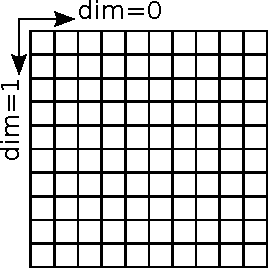
\includegraphics{pics/array.pdf}}
%\caption{{\small\label{fig:array}A two dimensional \nxfield\ before growing. }}
%\end{minipage}
%\hspace{0.01\linewidth}
%\begin{minipage}[t]{0.3\linewidth}
%\centering
%\resizebox{\linewidth}{!}{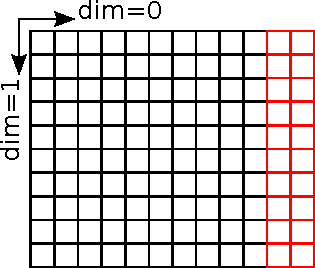
\includegraphics{pics/array_grow.pdf}}
%\caption{{\small\label{fig:array_grow}The \nxfield\ after growth along dimension
%$0$ by $2$ elements.}}
%\end{minipage}
%\hspace{0.01\linewidth}
%\begin{minipage}[t]{0.36\linewidth}
%\centering
%\resizebox{\linewidth}{!}{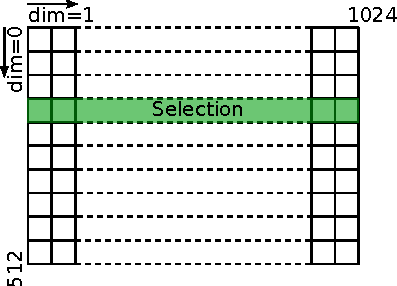
\includegraphics{pics/selection.pdf}}
%\caption{{\small\label{fig:selection}\nxselection\ object allow to read only 
%portions of an \nxfield. This is sometimes useful where one is not interested in
%the entire data.}}
%\end{minipage}
%\end{figure}
%%%============================================================================
\begin{figure}[tb]
\centering
\begin{minipage}[c]{0.3\linewidth}
\centering
\resizebox{\linewidth}{!}{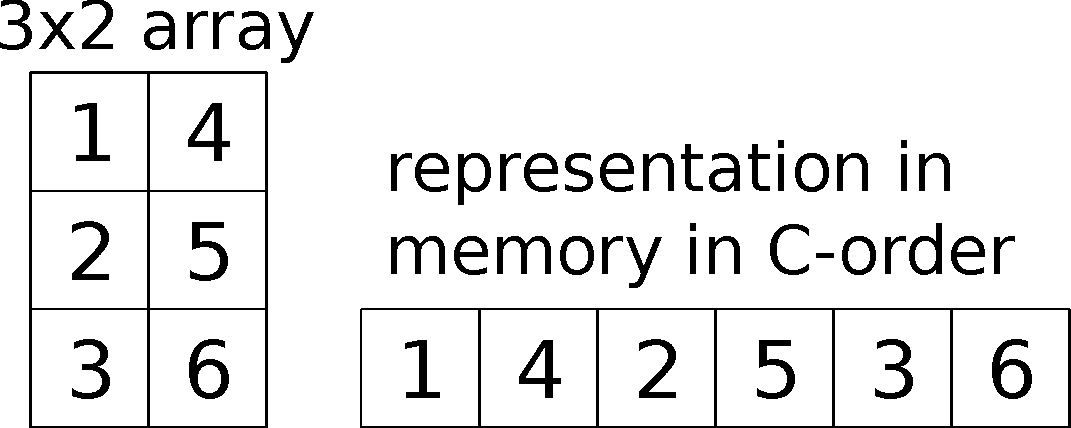
\includegraphics{pics/c-order.pdf}}
\end{minipage}
\hfill
\begin{minipage}[c]{0.68\linewidth}
\caption{{\small\label{fig:c_order}
\nxfield\ objects store data in C-order. This means that if the array is
unrolled in its linear representation the last index varies fastest. 
This examples shows how a $(3,2)$ array would look in its linear representation
using C-ordering.  }}
\end{minipage}
\end{figure}
%%%----------------------------------------------------------------------------
The most important class in \pninx\ is \nxfield\ which finally stores the data
of interest. Instances of \nxfield\ can be considered as multidimensional
arrays. Such an array is described by two quantities
\begin{enumerate}
\item its {\em rank} which is the number of dimensions
\item and its {\em shape} storing the number of elements along each
dimension
\end{enumerate}
In addition the type of the data must be known. As computer memory has no notion
of multidimensional structures data is stored in linear arrays. The
multidimensional index representing a particular index in the array is than
mapped on the linear index of the element in this array. There are basically two
types of such mappings: Fortran-ordering and C-ordering. In case of the former
one the first value of the multidimensional index varies fastest while in the
latter one it is the last value. \nxfield\ objects use C-ordering. 
Figure~\ref{fig:c_order} shows an example of how a $3\times 2$ array is mapped
onto a linear memory region. 
Unlike the original Nexus C-API \pninx\ provides no possibility to change this
behavior. As long as you stay in the world of C or  use array objects from
\pniutils\ this is no problem as they use the same ordering convention as
\pninx. However, you have to take this into account if you want to read data
from a Fortran program.

%%%----------------------------------------------------------------------------
\begin{figure}[tb]
\centering
\begin{minipage}[c]{0.25\linewidth}
\subfloat[Array before growth]{
\centering
\label{fig:array_growth:before}
\resizebox{\linewidth}{!}{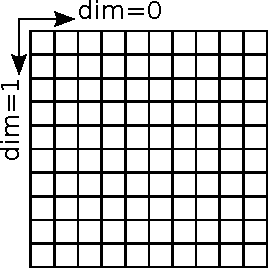
\includegraphics{pics/array.pdf}}
}
\end{minipage}
\hspace{0.01\linewidth}
\begin{minipage}[c]{0.3\linewidth}
\subfloat[Array after growth]{
\centering
\label{fig:array_growth:after}
\resizebox{\linewidth}{!}{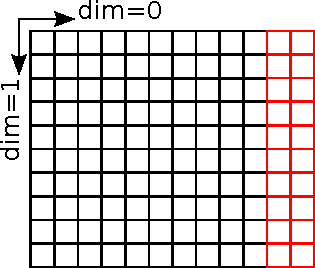
\includegraphics{pics/array_grow.pdf}}
}
\end{minipage}
\hfill
\begin{minipage}[c]{0.4\linewidth}
\caption{{\small\label{fig:array_growth}A 2-dimensional array before (a) and
after growth (b) by two elements along dimension 0. Note that the direction of a
dimension shown in the sketch does not give any information about its index
position. The index that varies fastest is that of dimension $1$ which runs in
vertical direction in this figure.}}
\end{minipage}
\end{figure}
%%%-----------------------------------------------------------------------------
The rank and the data-type of an instance or \nxfield\ are determined at the
time the object is created. However, the number of elements along each dimension
can be altered at any time during the lifetime of the object.
However, due to limitations of HDF5 the number of elements along each dimension
can only grow (deletion is not possible). 
Figure~\ref{fig:array_growth} depicts such a growth process of a $2$-dimensional 
\nxfield\ object. The original array shown in
Fig.~\ref{fig:array_growth:before} is extended by two elements as can be
obtained from Fig.~\ref{fig:array_growth:after}.


\subsection{Selections - partial IO}
%%%----------------------------------------------------------------------------
\begin{figure}[tb]
\centering
\begin{minipage}[c]{0.32\linewidth}
\centering
\subfloat[Simple selection]{
\label{fig:selection:no_stride}
\resizebox{\linewidth}{!}{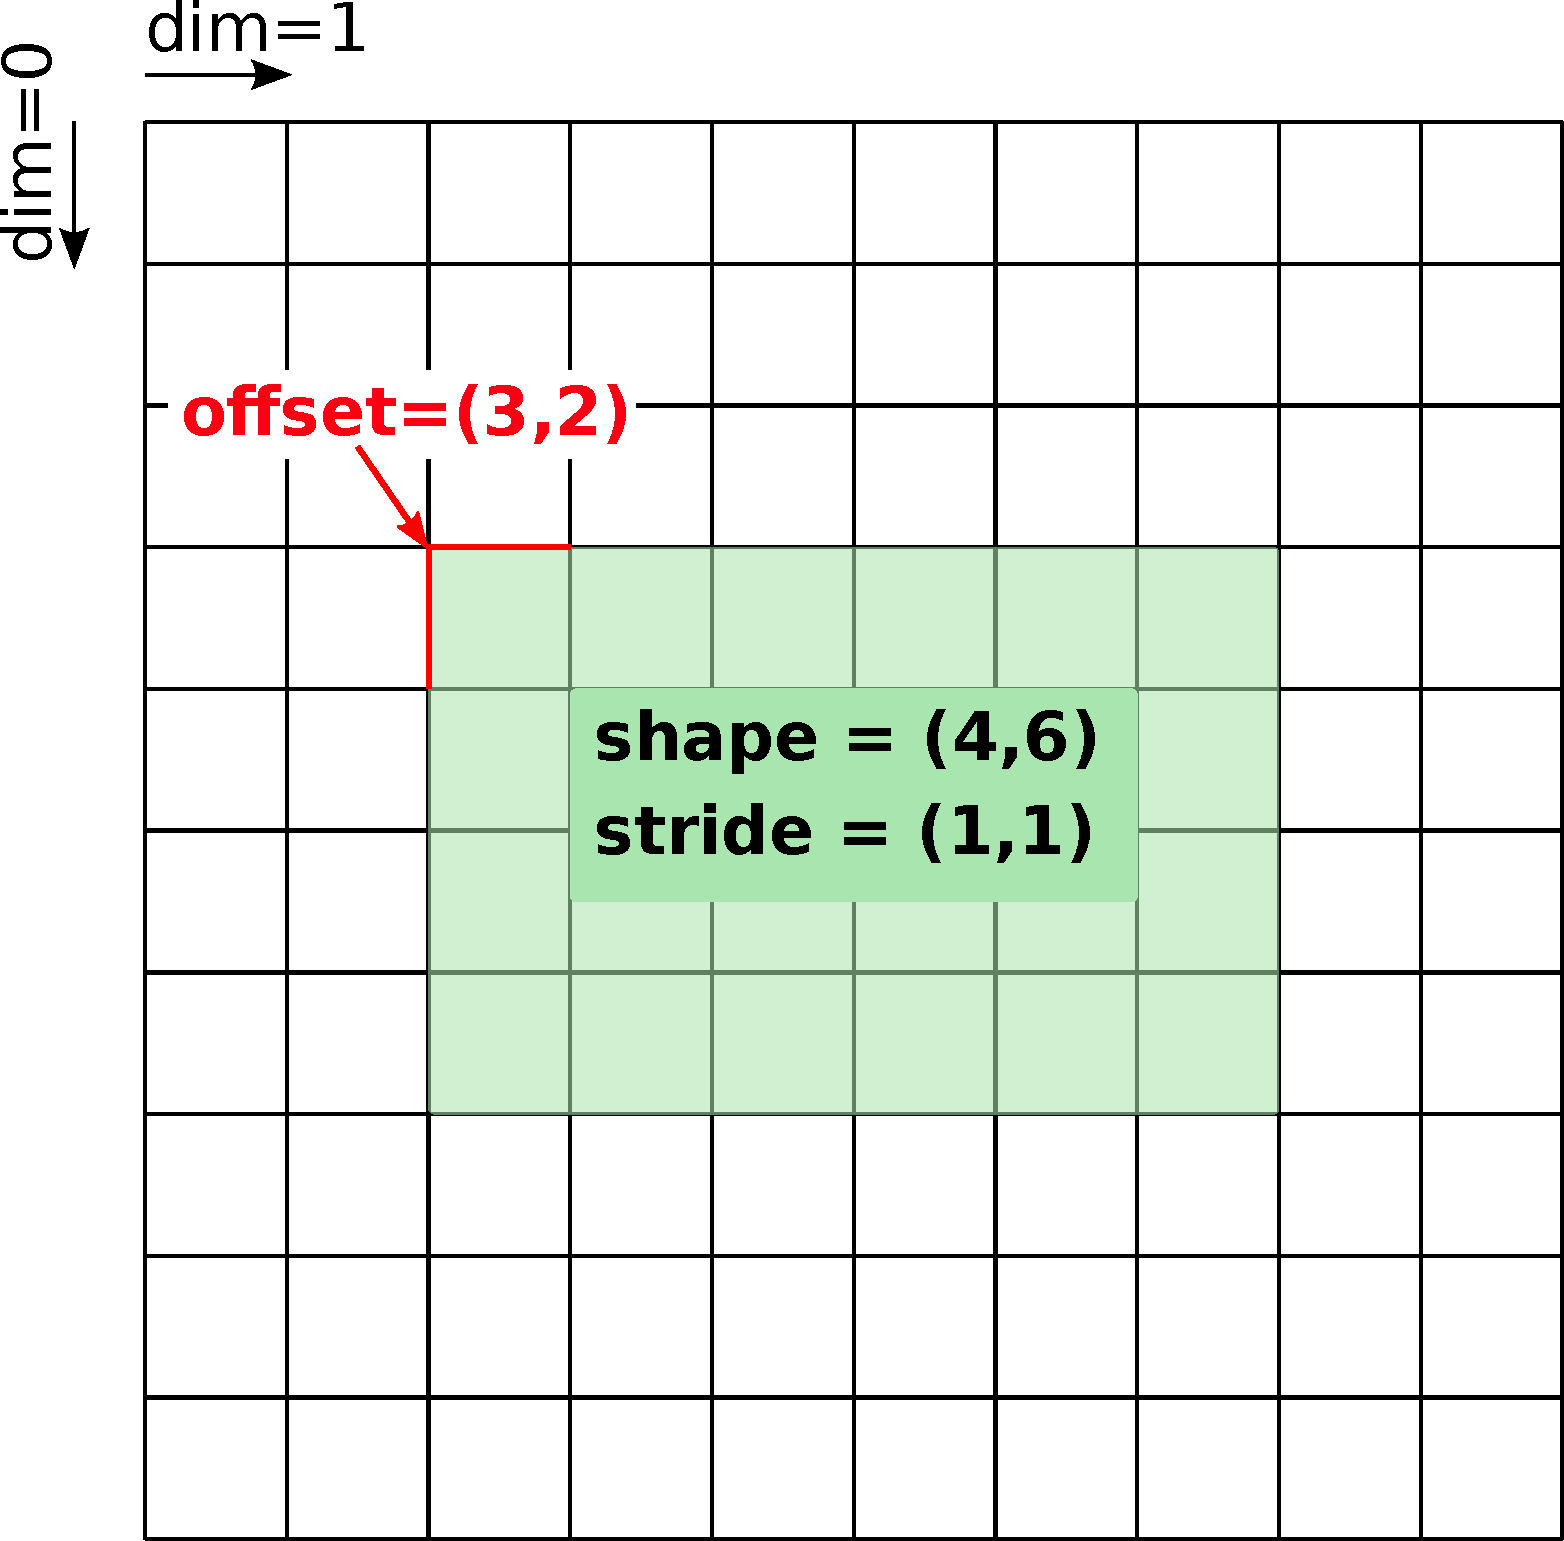
\includegraphics{pics/selection_2.pdf}}
}
\end{minipage}
\hspace{0.01\linewidth}
\begin{minipage}[c]{0.32\linewidth}
\centering
\subfloat[Selection with stride]{
\label{fig:selection:stride}
\resizebox{\linewidth}{!}{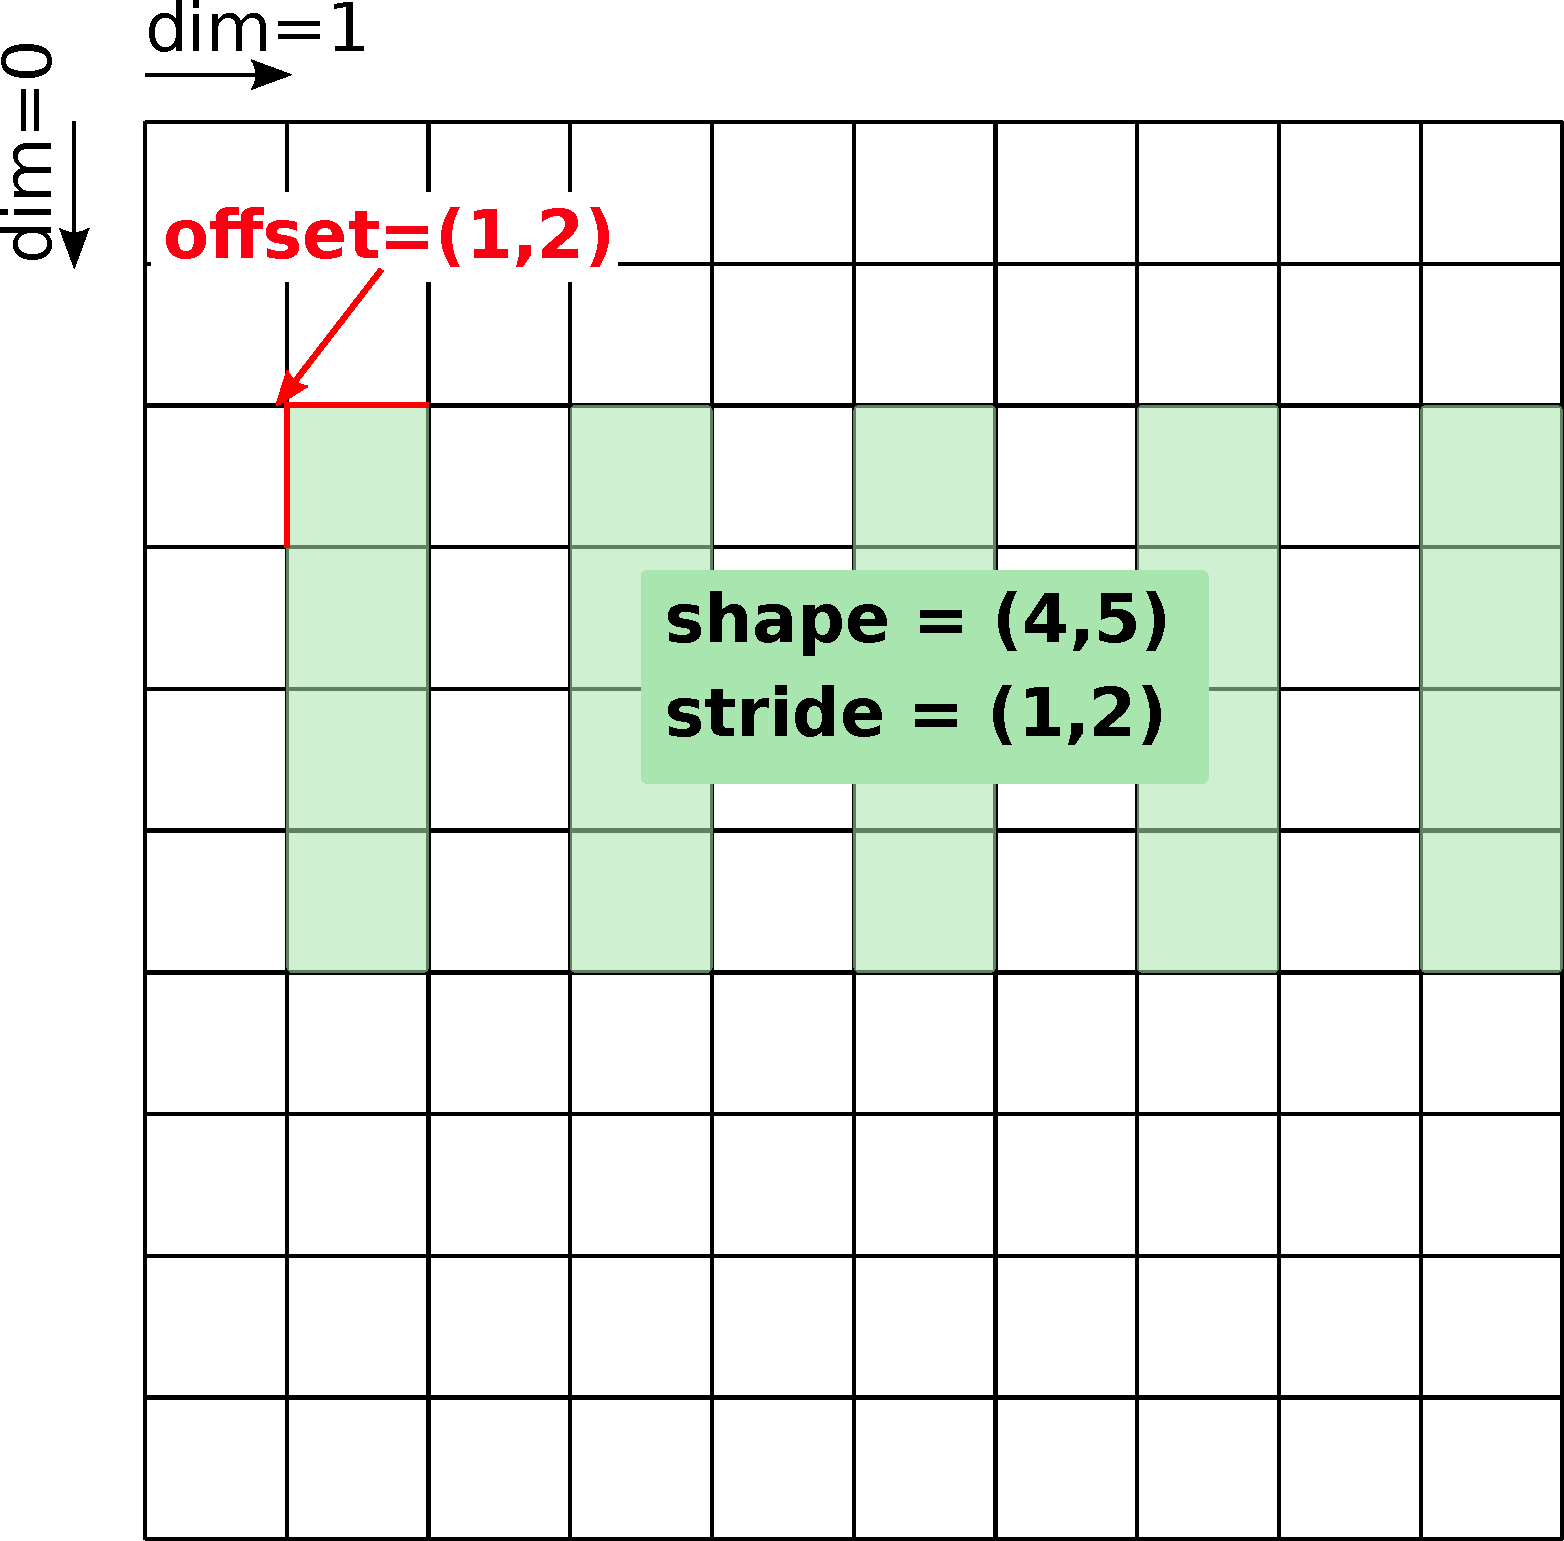
\includegraphics{pics/selection_3.pdf}}
}
\end{minipage}
\hspace{0.01\linewidth}
\begin{minipage}[c]{0.3\linewidth}
\caption{{\small\label{fig:selection}
Tow different selections applied to a $10\times 10$ \nxfield.
In (a) the selection has a uniform stride of $(1,1)$ selecting a continuous
region in the field. In (b) the stride is set to $(1,2)$ allowing to interleave
elements in the field. The shape of a selection describes the number of elements
along each of its dimensions. A selections offset describes its start in the
original field.}}
\end{minipage}
\end{figure}
%%%----------------------------------------------------------------------------
A utility class of particular importance is the \nxselection\ class. 
It allows IO access to parts of a field object. Selections are closely bound to
field objects. They can only be constructed by the {\tt selection()} factory
method of a field object and thus cannot be applied to other fields.
An instance of \nxselection\ is characterized by three quantities
\begin{enumerate}
    \item an {\em offset} which is the starting index of the selection in the
    original data field
    \item a {\em shape} determining the number of elements along each direction
    of the original field
    \item and a {\em stride} determining the spacing between the selected
    elements in the original data field.
\end{enumerate}
In Fig.~\ref{fig:selection} two examples for selections are shown. 
The rank of offset, stride, and shape of an array is equal to the rank of the
field to which the selection is bound. However, this does not necessarily mean
that the rank of the memory object from or to which data is written or read must
be equal the rank of the field or selection. 
One can for instance select a single element in a 3-dimensional field write the
content of a scalar value to this selection. 
We will see examples for this in later chapters.

\subsection{Chunks: contiguous in memory $\ne$ contiguous on disk}
%%%-----------------------------------------------------------------------------
\begin{figure}[tb]
\centering
\begin{minipage}[c]{0.68\linewidth}
\centering
\resizebox{\linewidth}{!}{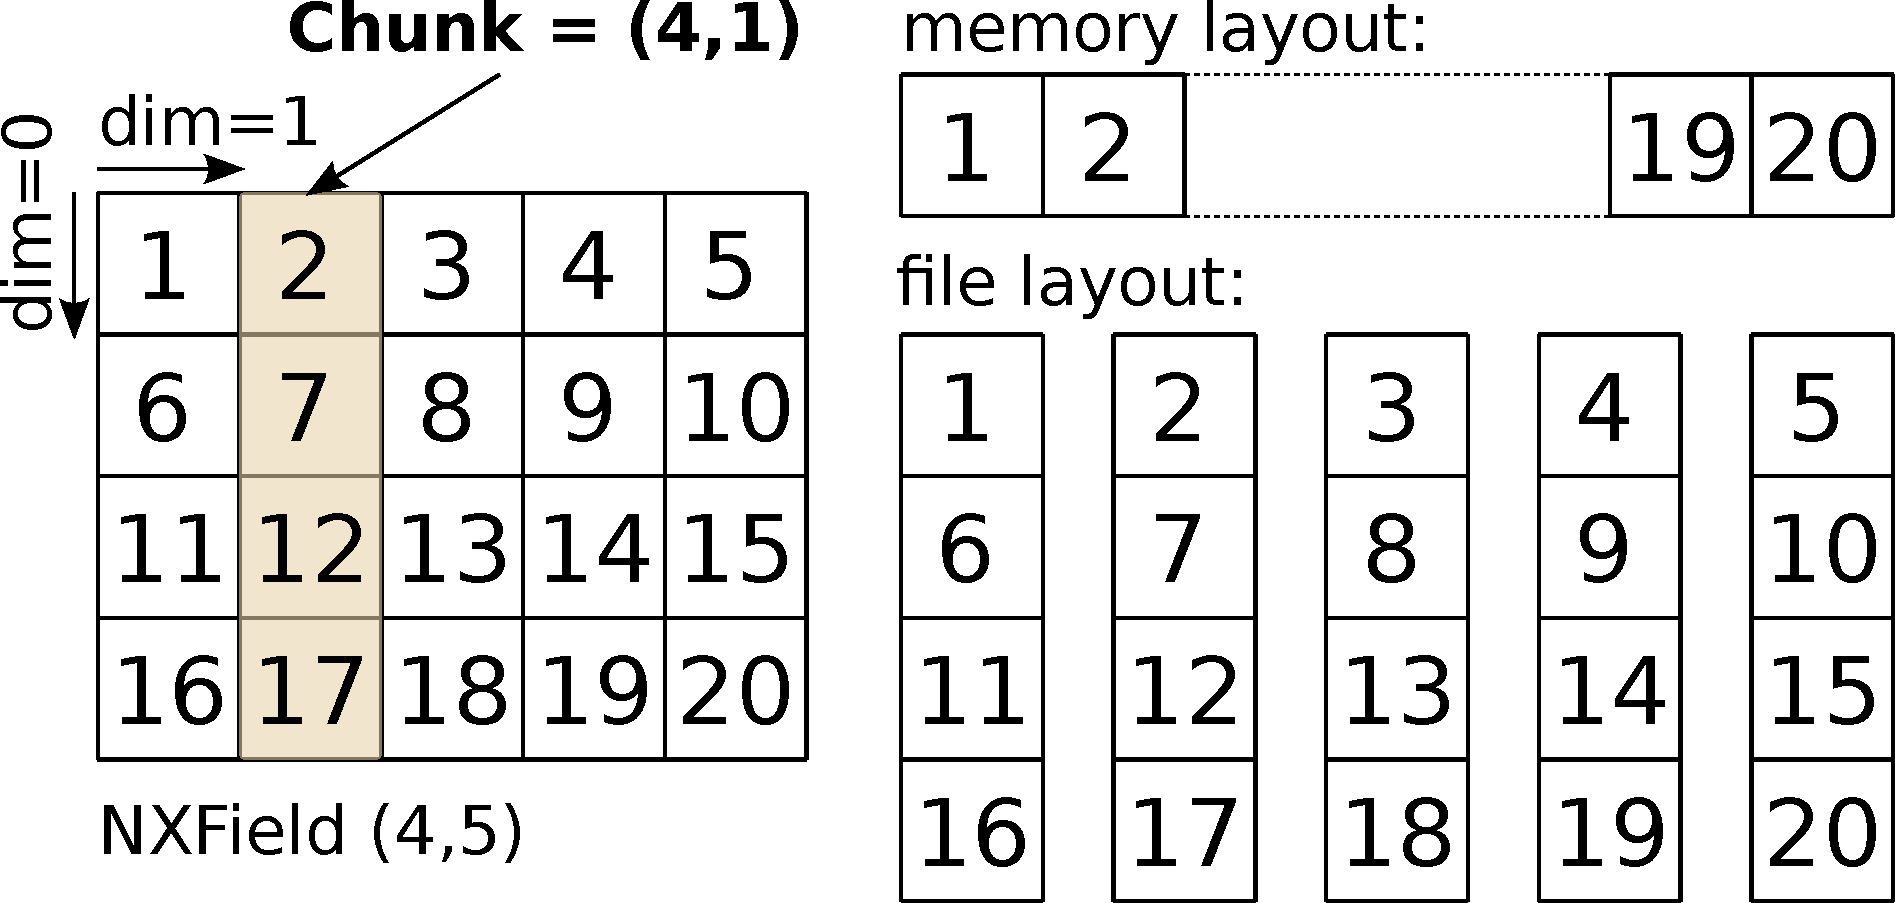
\includegraphics{pics/chunk.pdf}}
\end{minipage}
\hfill
\begin{minipage}[c]{0.3\linewidth}
\caption{{\small\label{fig:chunk}The chunk of an \nxfield\ object determines
which components of the multidimensional array reside contiguous on disk. 
As shown in this example this must not be the same components that are
contiguous in memory once the field has been read from disk.}}
\end{minipage}
\end{figure}
%%%------------------------------------------------------------------------------
The concept of chunks comes from the realm of HDF5 and has no counterpart in the
Nexus world. However, since the choice of chunks might significantly
increase data access performance \pninx\ provides the functionality to configure
chunks. A chunk describes the portion of data from a field that lies contiguous
on disk. As shown in Fig.~\ref{fig:chunk} these contiguous disk chunks must not
necessarily be the same contiguous regions than the memory representation of the
field.
It follows immediately from this considerations that it has great influence for
IO performance which components lie contiguous on disk and which not. 
This is particularly true if you use selections for IO. 
To clarify this lets have a look on a small example. We start again with the
field described in Fig.~\ref{fig:chunk} and assume furthermore that we want to
write data to this field by using a selection which represents a single strip of
data. The situation is depicted in Fig.~\ref{fig:chunk_io}.
In Fig.~\ref{fig:chunk_io_bad} the selection object lies perpendicular to the
chunk shape of the field to which data shall be written. 
In consequence every time data is written via the selection the library must
jump from one chunk to the next to write data. This is obviously not a very
clever solution. Indeed all chunks must be created once the write process
starts.
The situation in Fig.~\ref{fig:chunk_io_good} is more feasible. Here the shape
of the selection coincides with the shape of the field's chunk shape. 
When data is written through the selection object a single chunk can be filled
with contiguous data. Obviously this approach should be preferred over the
previous ones. Although I mentioned only writing data here, the same is true for
reading data back from the file. 
It can happen that the optimum chunk setups for reading and writing are mutually
exclusive. In such situations compromises are unavoidable. It is usually the
best approach to find the operations which is more important: reading or
writing.
 
%%%----------------------------------------------------------------------------
\begin{figure}[tb]
\centering
\begin{minipage}[c]{0.68\linewidth}
\centering
\subfloat[Chunk-selection-misaligned]{
\label{fig:chunk_io_bad}
\resizebox{\linewidth}{!}{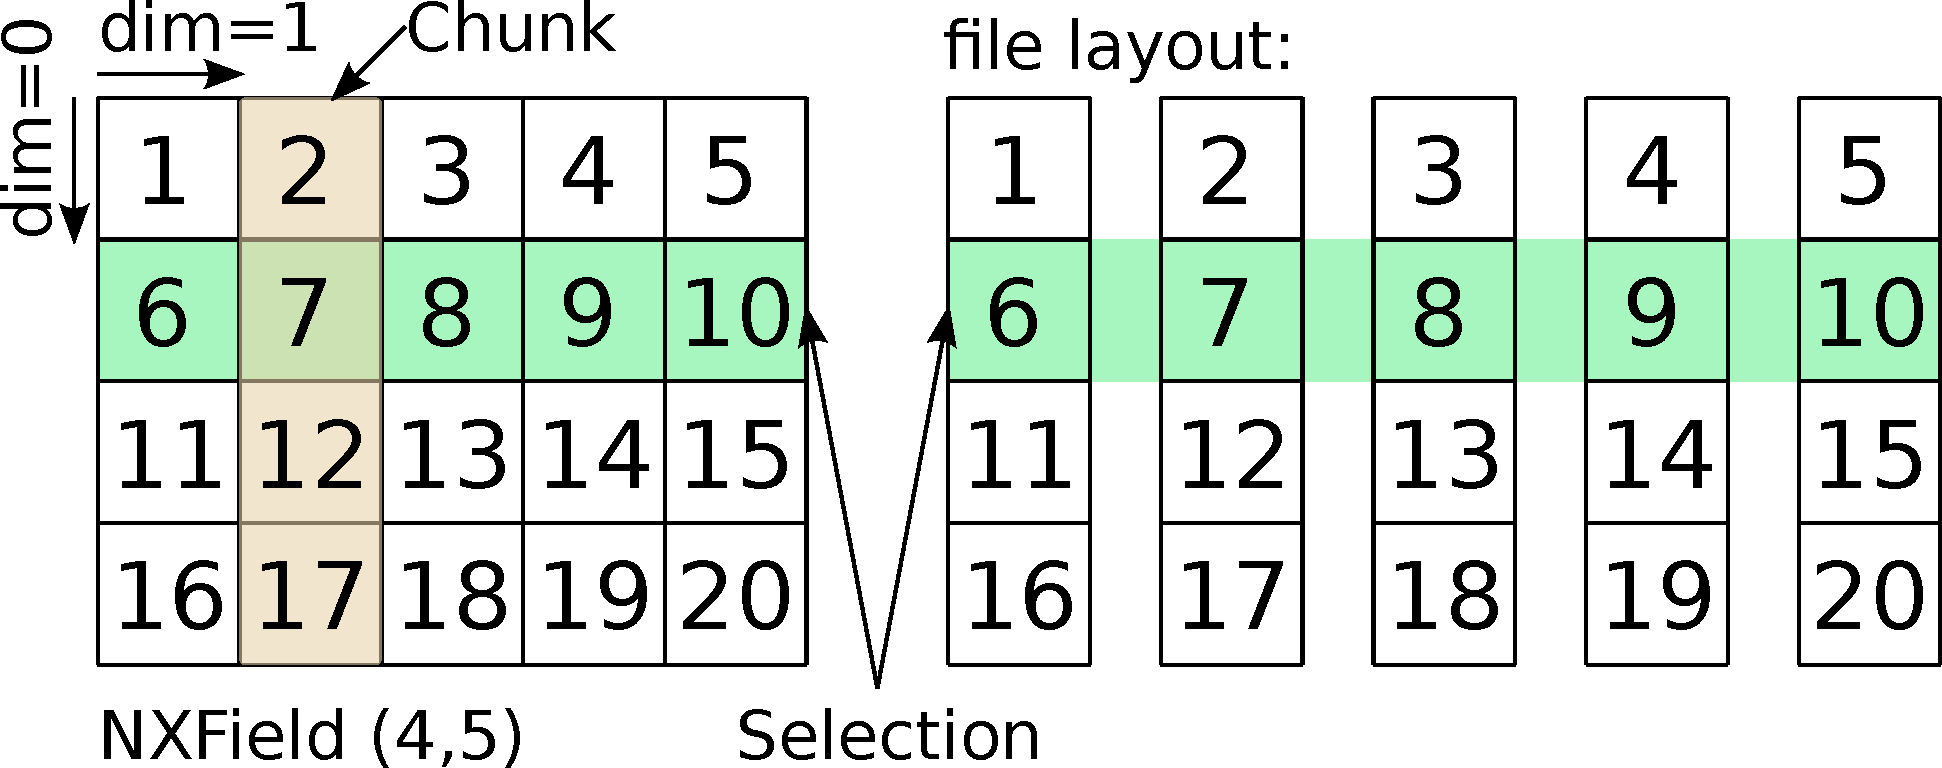
\includegraphics{pics/chunk_badio.pdf}}
}\\
\subfloat[Chunk-selection-aligned]{
\label{fig:chunk_io_good}
\resizebox{\linewidth}{!}{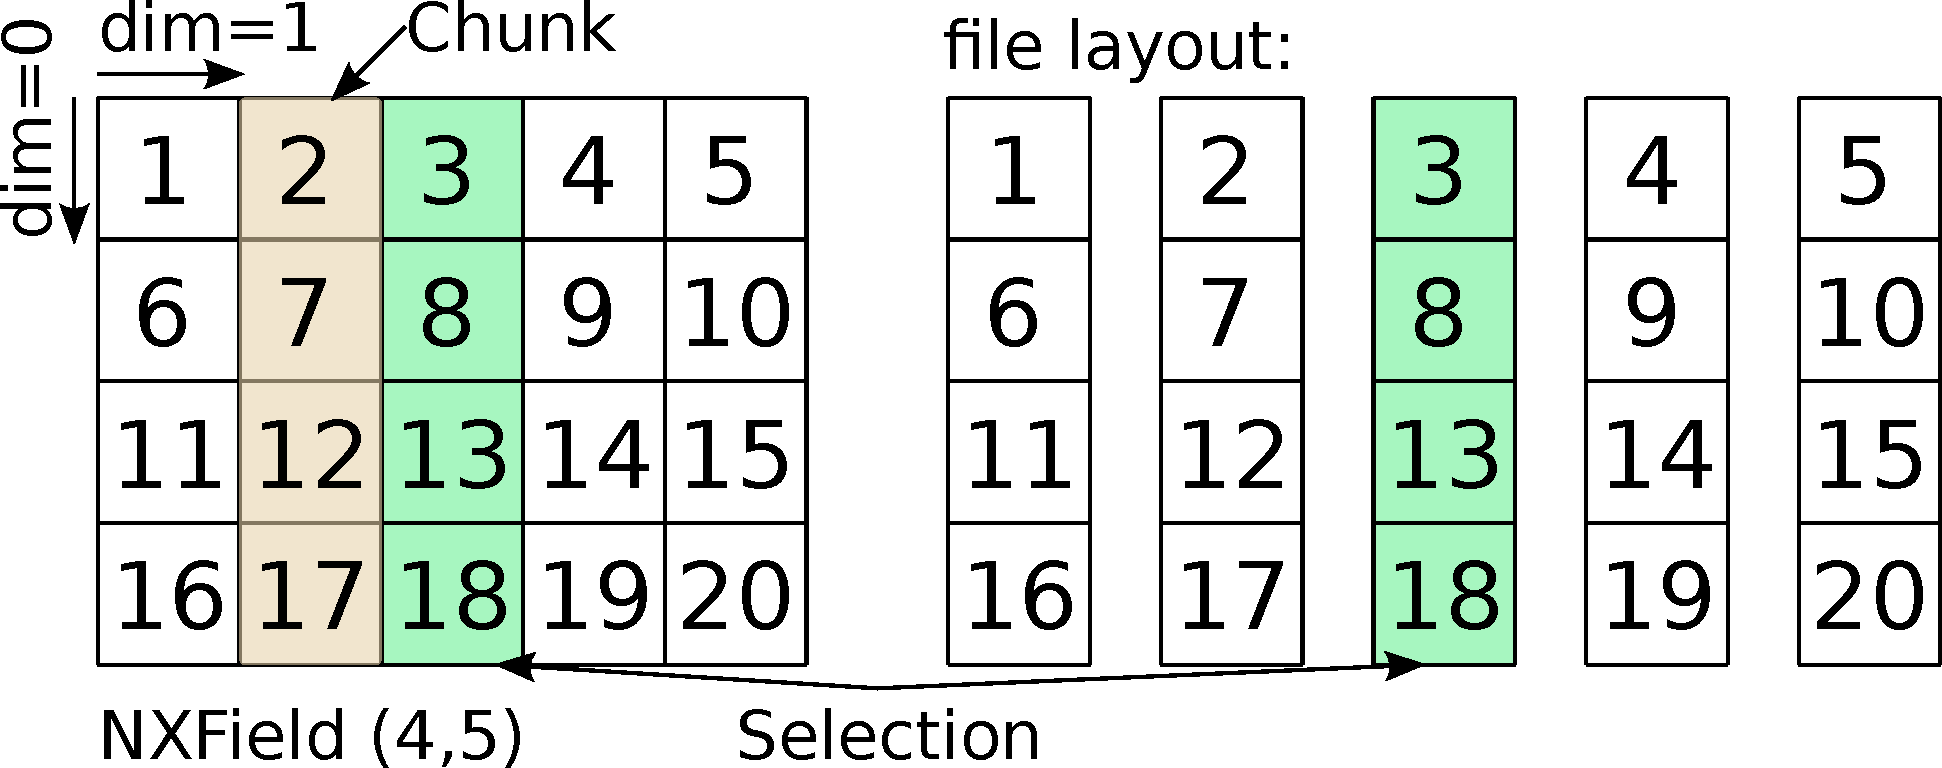
\includegraphics{pics/chunk_goodio.pdf}}
}
\end{minipage}
\hfill
\begin{minipage}[c]{0.3\linewidth}
\caption{{\small\label{fig:chunk_io}
Data IO using a selection on a 2-dimensional field where in (a) the selection is
perpendicular to the chunk shape of the field. In this case every time a
selection is written to disk the library must jump from one chunk to the next. 
This is obviously not the best approach for high performance.
The situation in (b) is much better. Here the selection shape coincides with the
chunk shape. When a selection is written a single chunk can be filled by the
library which is obviously easier than to jump from one chunk to the next for
every data value. This leads to much better performance than the approach in
(a).}}
\end{minipage}
\end{figure}
